\documentclass[12pt,a4paper]{book}
\usepackage[utf8]{inputenc} % Encodage UTF-8
\usepackage[french]{babel} % Langue française
\usepackage[T1]{fontenc}   % Encodage des caractères
\usepackage{amsmath}     % Package pour les mathématiques (utilisé ici pour des tableaux complexes)
\usepackage{amsfonts}
\usepackage{amssymb}
\usepackage[left=2cm,right=2cm,top=2cm,bottom=2cm]{geometry}
\usepackage{multirow} % Package pour fusionner les lignes
\usepackage{graphicx} % Pour insérer des images
\usepackage{array}           % Amélioration des tableaux
\usepackage{booktabs}        % Meilleure gestion des tableaux
\usepackage{hyperref}        % Liens hypertextes
\usepackage{pgfplots}
\usepackage{makeidx}
\usepackage{lmodern}
\author{Classe Master}
\linespread{1}

\begin{document}
%% Debut Page de garde
\begin{titlepage}
    \centering  
    
\includegraphics[width=3cm]{UP.jpg} \hspace{9cm}    
\includegraphics[width=3cm]{ENSPD.jpg}
     
   \textbf{\normalsize RÉPUBLIQUE DU BÉNIN} \\[0.2cm]
    ****** \\[0.2cm]

    \textbf{\normalsize UNIVERSITÉ DE PARAKOU} \\[0.2cm]
    ****** \\[0.2cm]

    \textbf{\normalsize ÉCOLE NATIONALE DE STATISTIQUE DE PLANIFICATION ET DE DÉMOGRAPHIE (ENSPD)} \\[0.2cm]
    ****** \\[0.2cm]

    \textbf{\normalsize {SOUTENANCE DE FIN D'ÉTUDES EN PLANIFICATION ET SUIVI-ÉVALUATION}} \\[0.5cm]
     
       \rule{\linewidth}{0.5mm}\\[0.2cm]
         \textbf{\large OPTIMISATION DES METHODES DE SUIVI-EVALUATION DANS LES PROJETS}
        \rule{\linewidth}{0.5mm} \\[0.8cm]

    \textbf{\normalsize Présenté par :} \textbf{Kamila H. Chimène AKPAKI} \\[1cm]

    % Image décoration
    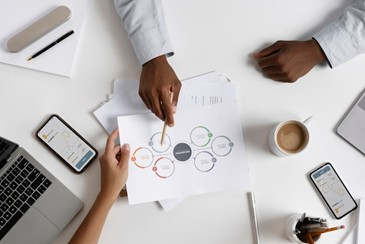
\includegraphics[width=10cm]{Image2.jpg} \\[1cm]
    
 \vfill
    \textbf{\normalsize Encadrant : Ph.D. George DJOHY} \\[1cm]

    \textbf{\normalsize ENSPD : 2/7/2025} \\[2cm]

\end{titlepage}
%% Fin de Page de garde

%%%Tableau Realisation de tableaux
\centering
\begin{table}[h!]%la précision sur le h! pour qu'il reste reste néccésairement sur une même page
\begin{tabular}{|c|c|c|c|}\hline
1&2&3&4\\
\hline
\multicolumn{2}{|c|}{blabla}&6&10\\\hline
&&9&11\\
\hline

\end{tabular}
\hspace{5cm}
\begin{tabular}{|c|c|c|c|}\hline
1&2&3&4\\
\hline
\multicolumn{2}{|c|}%fusion de deux collones ayant 2cm de large et contenant le message 'c'est ça'
{blabla}&6&10\\\cline{3-4}%puis on trace une ligne entre la 3è et la 4è colonne à l'endroit mis
\multicolumn{2}{|c|}{}
&9&11\\
\hline
\end{tabular}
\\
\\%crée des espaces verticales
\\
\begin{tabular}{|c|c|c|c|}\hline
1&2&3&4\\
\hline
\multicolumn{2}{|c|}{bla}
&6&10\\
\hline
&B&9&11\\
\hline
\end{tabular}
\hspace{5cm}
\begin{tabular}{|c|c|c|c|}\hline
1&2&3&4\\
\hline
\multirow{2}{2cm}{C'est ça}%fusion de deux ligne ayant 2cm de large et contenant le message 'c'est ça'
&&6&10\\\cline{2-4}
&B&9&11\\
\hline
\end{tabular}
\label{Table}
\caption{Titre de tables}
\end{table}
%%%Tableau Realisation de tableaux

%inserer une nouvelle page vierge
\newpage
\thispagestyle{empty}
la vie du bon coté

%insertion d'image
\begin{figure}[h]
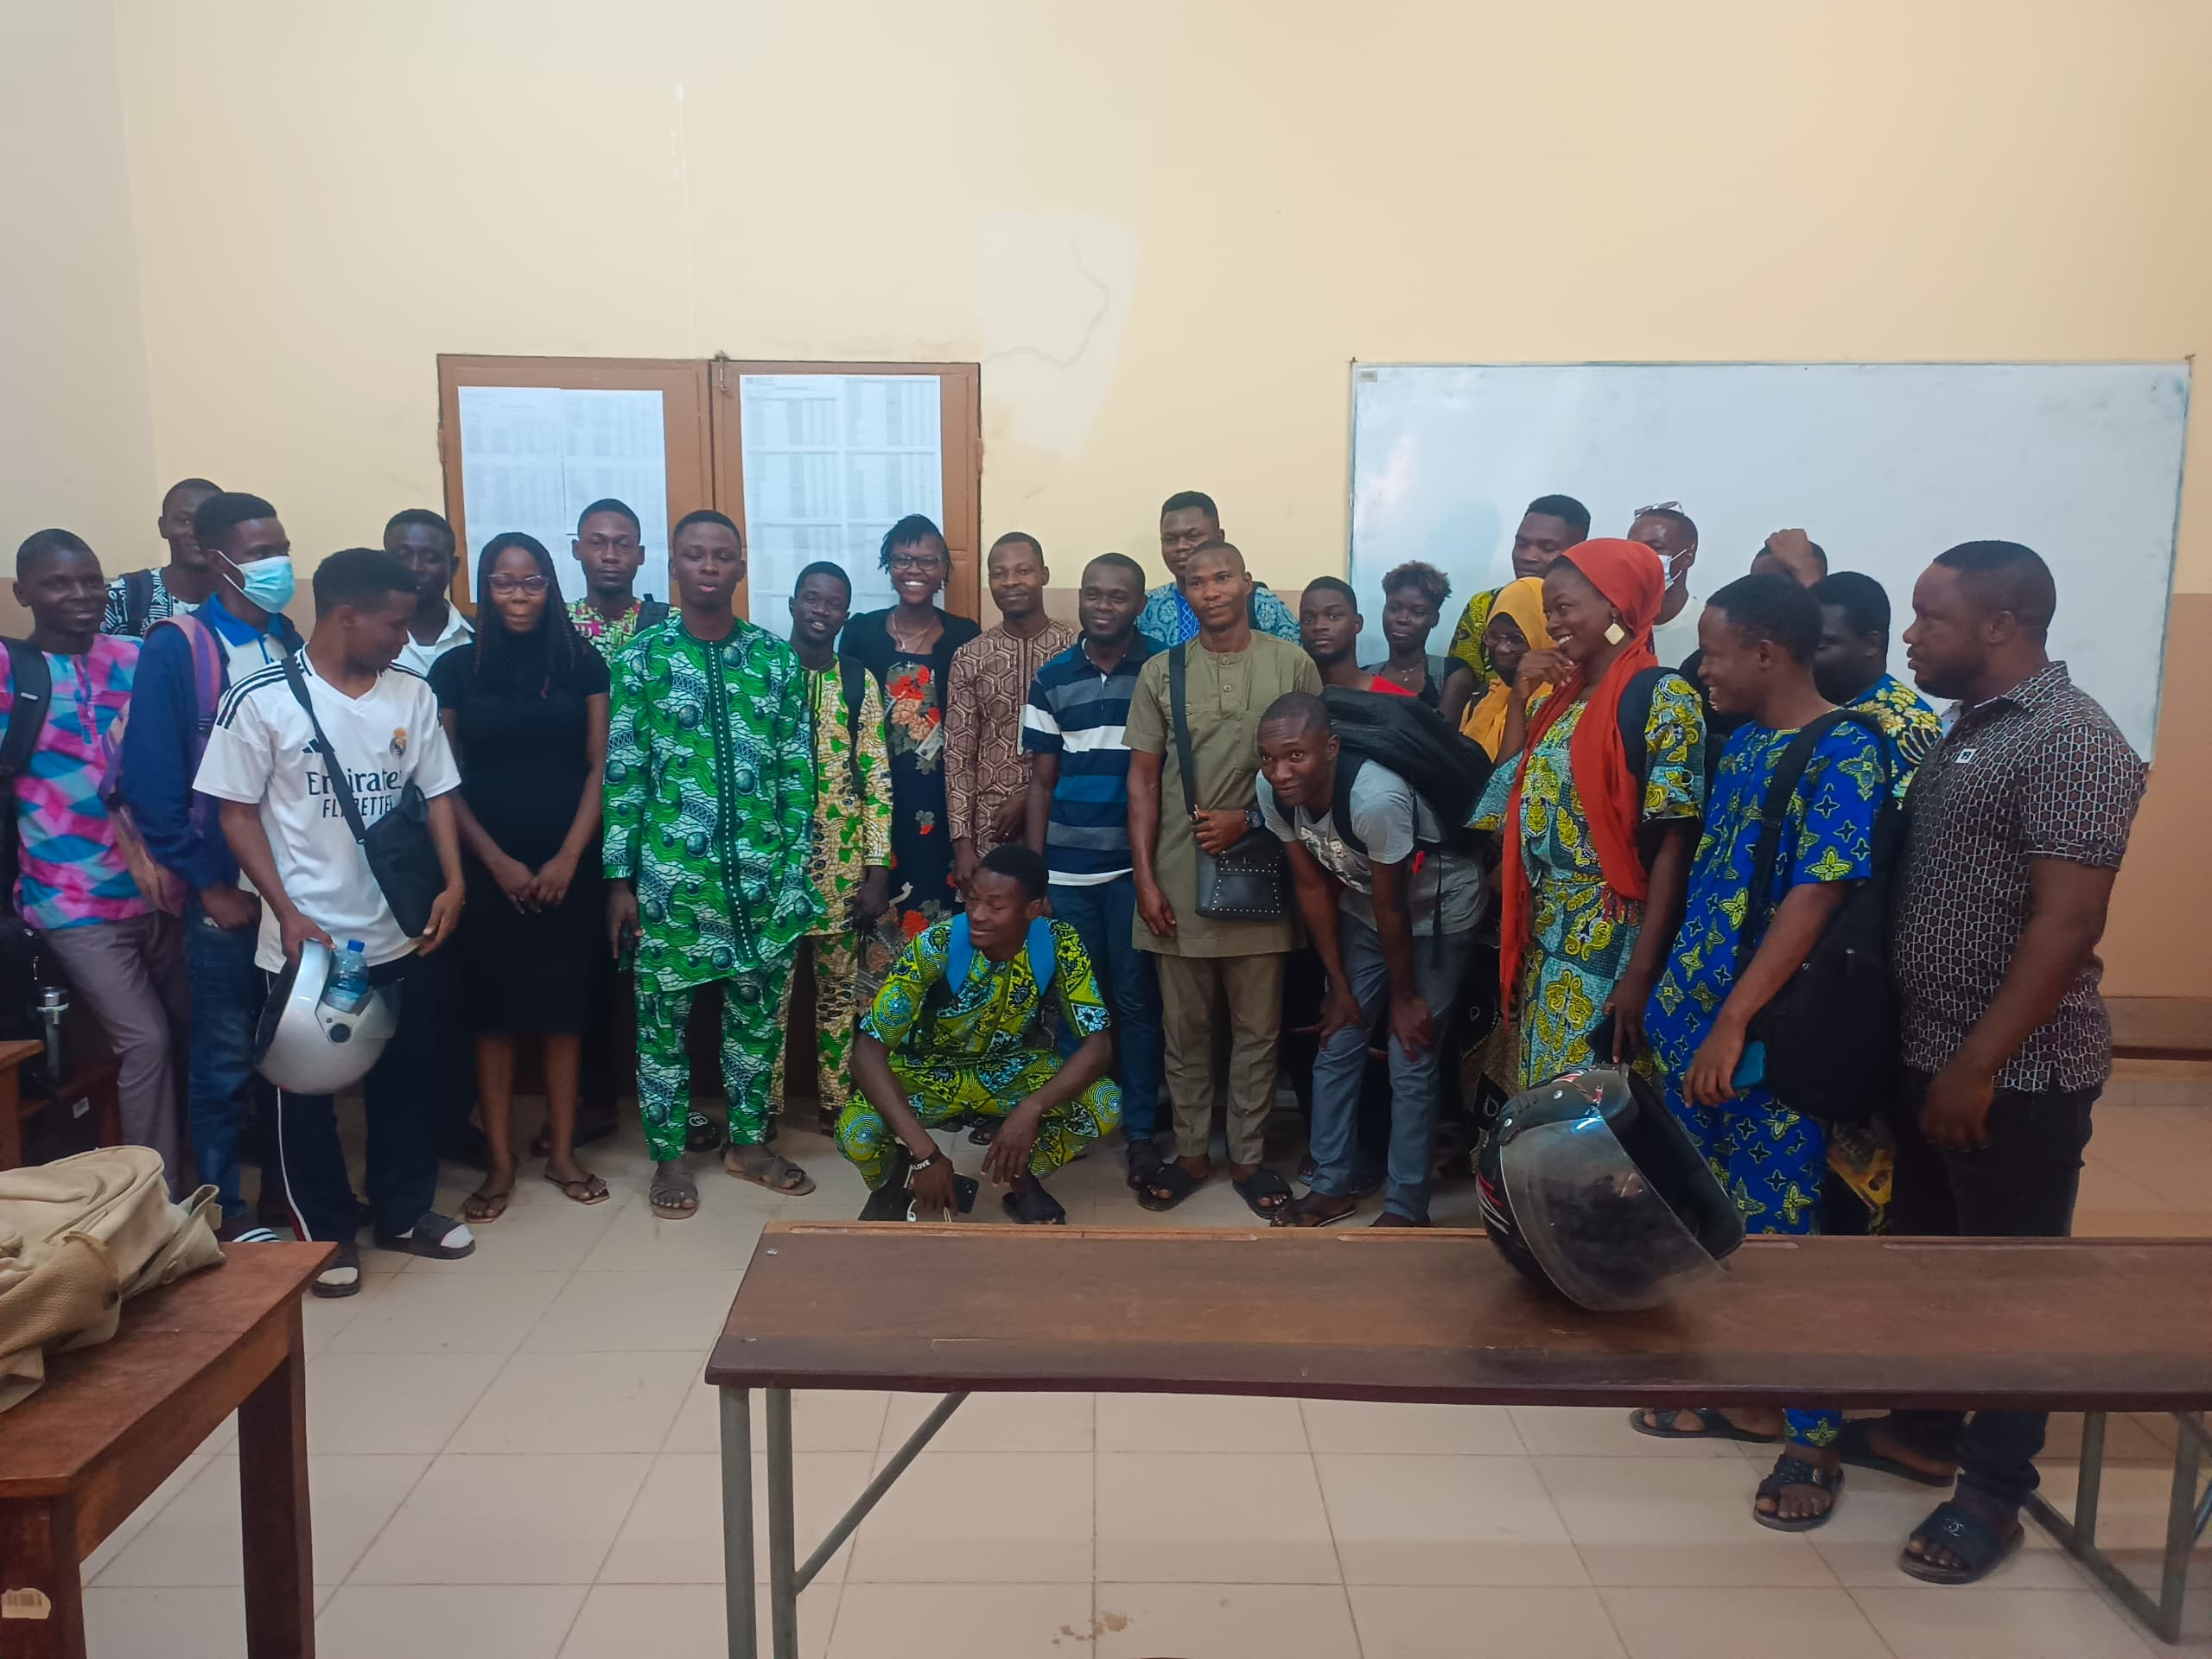
\includegraphics[scale=0.30]{aa.jpg}%scale correspond à l'échelle dont on veux le reduire 
\label{Photo}%nom à mettre en bas de l'image
\caption{photo de classe}%titre à ajouter à l'image
\end{figure}

%document : introduction au Latex
%\maketitle % Génère le titre
\section{Introduction}

\section*{Introduction à \LaTeX} % Section non numérotée

Dans le monde de la rédaction scientifique et technique, \LaTeX{} s’impose comme un outil incontournable pour produire des documents de haute qualité. Contrairement aux éditeurs de texte classiques comme \textbf{Microsoft Word}, qui reposent sur le principe du \textit{WYSIWYG} (\textit{What You See Is What You Get}), \LaTeX{} fonctionne sur un système de \textbf{balisage} où l’utilisateur écrit du \textbf{code} décrivant la structure du document. Ce processus permet d’obtenir une mise en page \textbf{automatisée, propre et cohérente}, idéale pour les \textbf{thèses, articles scientifiques, rapports et livres}.  

Développé à partir de \textbf{TeX} par \textbf{Leslie Lamport}, \LaTeX{} offre de nombreux avantages, notamment une \textbf{gestion avancée des références bibliographiques}, une \textbf{prise en charge efficace des formules mathématiques}, ainsi qu’un \textbf{alignement automatique des tableaux et figures}. Son approche modulaire permet également de \textbf{structurer facilement des documents longs} sans rencontrer de problèmes de mise en page.  

Bien que l’apprentissage de \LaTeX{} puisse sembler intimidant au début, il se révèle être un outil \textbf{puissant, flexible et largement utilisé} dans le monde académique et scientifique. Grâce à des éditeurs comme \textbf{TeXmaker, Overleaf ou MiKTeX}, il est désormais plus accessible et intuitif pour les utilisateurs souhaitant produire des documents professionnels avec une \textbf{qualité typographique irréprochable}.  


\section{Texte et structure}]
Voici un paragraphe de texte normal.  
On peut aussi écrire en \textbf{gras}, en \textit{italique} ou en \underline{souligné}.  

% Informations du document
\title{Avantages de \LaTeX{} par rapport à Word}
\maketitle % Génère automatiquement le titre

\section{Generalite} % Titre principal de niveau 1
\LaTeX{} est un langage de composition de documents très puissant, 
particulièrement adapté aux travaux scientifiques et techniques. 
Contrairement à Word, qui repose sur le WYSIWYG (What You See Is What You Get), 
\LaTeX{} fonctionne selon un principe de séparation entre le contenu et la mise en forme. 
Cela apporte plusieurs avantages.

\section{Avantages de \LaTeX{} par rapport à Word}

\subsection{Qualité typographique supérieure} % Sous-titre (niveau 2)
\LaTeX{} produit des documents avec une mise en page professionnelle, 
particulièrement adaptée aux mathématiques et aux documents scientifiques.

\subsection{Automatisation de la mise en page}
Grâce à \LaTeX{}, l’utilisateur n’a pas à se soucier de la mise en forme. 
Tout est géré automatiquement (espacement, justification, placement des images, gestion des références.etc..).

\subsection{Gestion avancée des références et des bibliographies}
Avec des packages comme \texttt{biblatex}, \LaTeX{} permet de gérer facilement 
des bibliographies et des citations de manière standardisée.

\subsection{Facilité pour écrire des formules mathématiques}
Equation mathématique
\begin{equation}
    E = mc^2
E = \int_{a}^{b} x f(x) \,dx
\end{equation}

\subsection{Utilisation des tableaux et des figures bien structurés}
Avec \LaTeX{}, les tableaux et figures sont numérotés et placés intelligemment dans le document.

Insertion d'image avec légende
\begin{figure}[h]
    \centering
    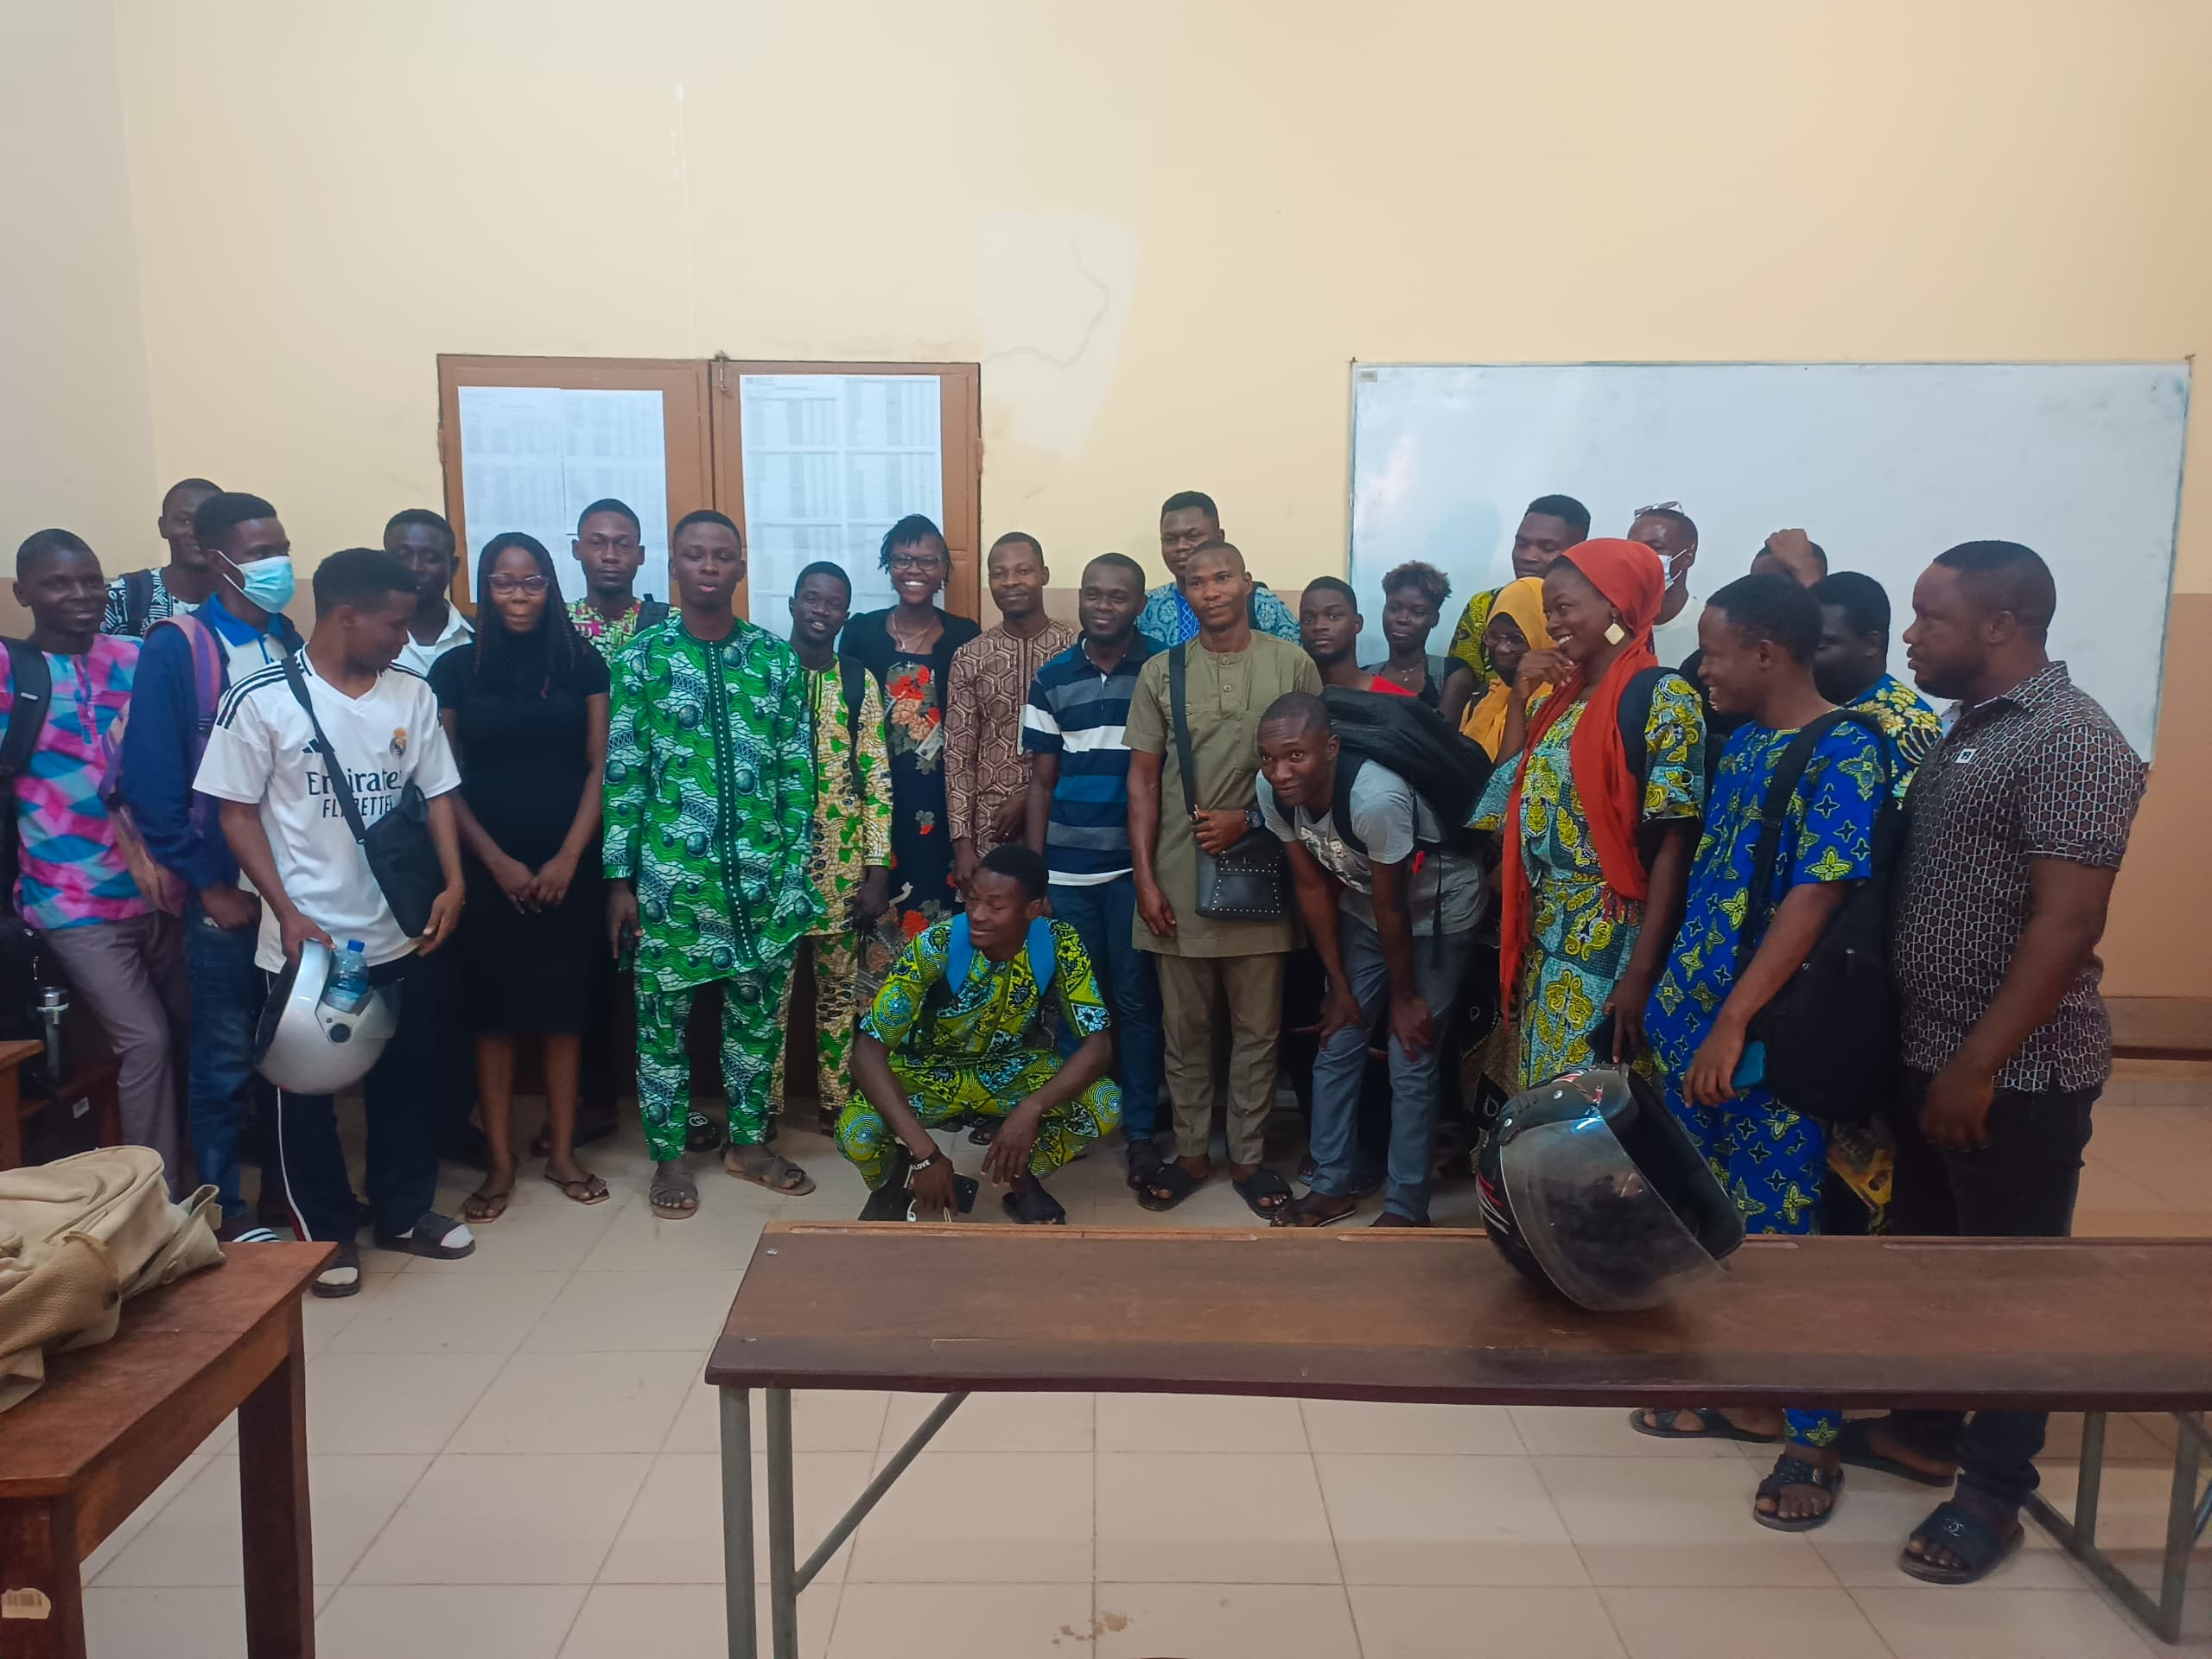
\includegraphics[width=0.5\textwidth]{aa.jpg} % Remplace "aa.jpg" par le nom de ton image
    \caption{Etudiant du Master 1 Capturer avec le Dr DJOHY}
    \label{fig:Etudiant du Master 1 2024-2025} % Permet de référencer l'image dans le texte
\end{figure}

\subsection{Meilleure gestion des longs documents}
\LaTeX{} est conçu pour des documents volumineux (thèses, livres, rapports). 
Il gère parfaitement les chapitres, annexes, tables des matières et index.

\subsection{Versionnage et collaboration facilitées}
Contrairement à Word, les fichiers \LaTeX{} sont en **texte brut** et peuvent être suivis avec des outils comme Git, ce qui facilite la collaboration et le suivi des modifications.

\subsection{Personnalisation et extensibilité}
Avec une grande variété de packages, \LaTeX{} permet d’ajouter des fonctionnalités avancées, 
comme les diapositives (\texttt{beamer}), les dessins vectoriels (\texttt{TikZ}), et bien plus encore.

\section{Conclusion} % Dernière section
En résumé, \LaTeX{} est une alternative puissante à Word, 
particulièrement adaptée aux documents scientifiques et techniques, 
grâce à sa flexibilité, sa qualité typographique et son automatisation avancée.

\title{Comportements à adopter pour atteindre un objectif}  % Titre 
\maketitle  % Génère le titre

\section{Comportements à adopter pour atteindre un objectif}

\begin{enumerate} %[label=\textbf{\arabic*.}]  % Liste numérotée
\item \textbf{Fixer des objectifs clairs et précis}
    \begin{itemize}  % Liste à puces
       \item[$\bullet$]\textbf{Définir des objectifs spécifiques} : Soyez précis sur ce que vous voulez accomplir (par exemple, au lieu de dire "Je veux être en forme", dites "Je veux perdre 5 kg en 3 mois").
        \item[$\bullet$] \textbf{Établir des critères de mesure} : Il est essentiel de pouvoir évaluer vos progrès (ex : "Je vais mesurer mon poids chaque semaine").
\item[$\bullet$] \textbf{Rendre les objectifs réalisables} : Assurez-vous que vos objectifs sont réalisables avec les ressources disponibles (temps, budget, etc.).
    \end{itemize}

   \item \textbf{Planifier et structurer son temps}
    \begin{itemize}
        \item[$\bullet$]\textbf{Créer un plan d'action} : Divisez votre objectif en tâches concrètes et planifiez-les sur une période spécifique (ex : chaque mois, chaque semaine, chaque jour).
        \item[$\bullet$]\textbf{Prioriser les actions importantes} : Concentrez-vous d'abord sur les tâches qui auront le plus grand impact pour atteindre l'objectif.
        \item [$\bullet$]\textbf{Prévoir des moments de réévaluation} : Faites régulièrement le point pour ajuster votre plan si nécessaire.
    \end{itemize}

       \item \textbf{Rester discipliné et persévérer}
    \begin{itemize}
        \item [$\bullet$]\textbf{Être constant dans l'effort} : Maintenez une routine régulière sans vous laisser distraire par des obstacles mineurs.
        \item [$\bullet$]\textbf{Gérer la procrastination} : Identifiez les causes de votre procrastination et adoptez des techniques comme le découpage des tâches ou la méthode Pomodoro pour rester motivé.
        \item[$\bullet$] \textbf{Ne pas se laisser décourager par les échecs} : Les échecs font partie du processus d'apprentissage. Considérez-les comme des opportunités de progression.
    \end{itemize}

  \item \textbf{Maintenir une attitude positive}
    \begin{itemize}
        \item [$\bullet$]\textbf{Visualiser le succès} : Imaginez régulièrement que vous atteignez votre objectif. Cette visualisation vous aidera à rester motivé.
        \item [$\bullet$]\textbf{Pratiquer l'autocompassion} : Soyez bienveillant envers vous-même, surtout lorsque vous rencontrez des difficultés.
        \item [$\bullet$]\textbf{Entourez-vous de personnes positives} : Évitez les personnes qui vous démoralisent et cherchez celles qui vous soutiennent.
    \end{itemize}

   \item \textbf{S'adapter et apprendre des erreurs}
    \begin{itemize}
        \item [$\bullet$]\textbf{Faire des ajustements si nécessaire} : Si quelque chose ne fonctionne pas, soyez prêt à adapter votre approche ou vos méthodes pour avancer.
        \item [$\bullet$]\textbf{Tirer des leçons des échecs} : Analysez les erreurs pour comprendre ce qui n'a pas fonctionné et trouver des solutions pour éviter de les répéter.
        \item [$\bullet$]\textbf{Chercher de nouvelles connaissances} : N'ayez pas peur d'apprendre de nouvelles compétences ou d'acquérir de nouvelles informations pour améliorer vos chances de succès.
    \end{itemize}

   \item \textbf{Gérer son énergie et son bien-être}
    \begin{itemize}
        \item [$\bullet$]\textbf{Prendre soin de sa santé physique et mentale} : Une bonne alimentation, de l'exercice, et un sommeil de qualité sont essentiels pour maintenir votre énergie et votre productivité.
        \item [$\bullet$]\textbf{Prendre des pauses régulières} : Le repos est nécessaire pour rester efficace et éviter l'épuisement.
        \item [$\bullet$]\textbf{Éviter le stress excessif} : Pratiquez des techniques de relaxation comme la méditation ou la respiration profonde pour rester calme et concentré.
    \end{itemize}

 \item \textbf{Mesurer et célébrer les progrès}
    \begin{itemize}
        \item [$\bullet$]\textbf{Suivre les progrès régulièrement} : Évaluez vos progrès par rapport aux objectifs fixés pour voir si vous êtes sur la bonne voie.
        \item [$\bullet$]\textbf{Célébrer chaque petite victoire} : Chaque étape franchie est un succès. Célébrez même les petites réalisations pour maintenir la motivation.
        \item [$\bullet$]\textbf{Revoir l'objectif final} : Gardez toujours en tête l'objectif ultime et pourquoi il est important pour vous.
    \end{itemize}
      \item \textbf{Rester flexible et ouvert aux opportunités}
    \begin{itemize}
        \item [$\bullet$]\textbf{Savoir saisir les opportunités imprévues} : Parfois, de nouvelles opportunités se présentent de manière inattendue. Soyez ouvert à les explorer si elles peuvent aider à atteindre votre objectif.
        \item [$\bullet$]\textbf{Accepter le changement} : La vie est imprévisible. Être prêt à ajuster vos plans en fonction de nouvelles circonstances est une compétence importante.
    \end{itemize}
    
    % En **LaTeX**, il existe plusieurs façons de personnaliser les **puces** (les symboles utilisés pour les éléments de listes) dans les environnements `itemize`. Voici quelques-unes des puces les plus courantes et comment les utiliser :

% 1. **Puces par défaut** (tirets) 
Ces puce peuvent etre utilisée dans l'environnement `itemize`.``latex
\begin{itemize}
    \item Premier élément
    \item Deuxième élément
\end{itemize}%Cela produit des tirets (ou points) devant chaque item.

% 4. **Puces rondes et pleines (●)**
%Utilise `\(\bullet\)` pour obtenir une puce ronde pleine :```latex
\begin{itemize}
    \item[$\bullet$] Premier élément
    \item[$\bullet$] Deuxième élément
\end{itemize}
% 5. **Flèche vers la droite (→)**
%Si tu préfères une flèche, tu peux utiliser un symbole comme `\(\rightarrow\)` :```latex
\begin{itemize}
    \item[$\rightarrow$] Premier élément
    \item[$\rightarrow$] Deuxième élément
\end{itemize}
% 6. **Puces avec des caractères spéciaux**Tu peux aussi insérer des caractères spéciaux comme des étoiles ou autres :``latex
\begin{itemize}
    \item[$\star$] Premier élément
    \item[$\star$] Deuxième élément
\end{itemize}
 % 7. **Puces personnalisées avec `enumitem`**Le package **`enumitem`** permet de personnaliser entièrement l'apparence des puces, y compris leur forme et leur taille. Par exemple :latex
% 8. **Autres symboles personnalisés**Tu peux aussi définir n'importe quel symbole comme puce, comme des étoiles, des cercles, des croix, etc. Exemple avec un cercle : il suffit de mettre le nom du symbol en anglais [$\nom du symbol en anglai$]
\begin{itemize}
    \item[$\circ$] Premier élément
    \item[$\circ$] Deuxième élément
\end{itemize}
% Résumé des symboles de puce courants :

% **$\bullet$** : Point plein.
%-**$\circ$** : Cercle vide.
% **$\square$** : Carré vide.
% **$\blacktriangle$** : Triangle plein.
% **$\star$** : Étoile.
% **$\rightarrow$** : Flèche droite.
% **$\diamond$** : Losange.
\end{enumerate}

\section{Numerotation et Sous-numérotation}
\begin{enumerate}
    \item UNIVERSITE DE PARAKOU
    \begin{enumerate}
        \item ECOLE NATIONALE DE STATISTIQUE, DE PLANIFICATION ET DE DEMOGRAPHIE
        \item CLASSE MASTER
    \end{enumerate}
\end{enumerate}

\section{Effectif de setudiants du master 1 regrouper par categorie}
Voici un tableau simple :

\begin{table}[ht]
\centering
\begin{tabular}{|l|c|c|c|}
\hline
\textbf{Row Labels} & \textbf{DISTANTIEL} & \textbf{PRESENTIEL} & \textbf{Grand Total} \\
\hline
\textbf{PSE}        & 24                 & 18                 & 42                  \\
\hline
\textbf{F}          & 2                  & 5                  & 7                   \\
\hline
\textbf{M}          & 22                 & 13                 & 35                  \\
\hline
\textbf{SA}         & 7                  & 15                 & 22                  \\
\hline
\textbf{F}          & -                  & 6                  & 6                   \\
\hline
\textbf{M}          & 7                  & 9                  & 16                  \\
\hline
\textbf{Grand Total} & 31                 & 33                 & 64                  \\
\hline
\end{tabular}
\caption{Tableau des comptages de "NOM ET PRENOMS" selon DISTANTIEL et PRESENTIEL}
\end{table}

% Tableau simple avec trois colonnes et trois lignes
\begin{tabular}{|c|c|c|}
\hline
Colonne 1 & Colonne 2 & Colonne 3 \\ % Première ligne de titres
\hline
Ligne 1 & Donnée 1 & Donnée 2 \\ % Première ligne de données
\hline
Ligne 2 & Donnée 3 & Donnée 4 \\ % Deuxième ligne de données
\hline
Ligne 3 & Donnée 5 & Donnée 6 \\ % Troisième ligne de données
\hline
\end{tabular}

\vspace{1cm} % Espace vertical entre les tableaux

% Tableau avec fusion de colonnes
\begin{tabular}{|c|c|c|}
\hline
Colonne 1 & \multicolumn{2}{c|}{Fusion des Colonnes 2 et 3} \\ % Fusion des deux colonnes 2 et 3
\hline
Ligne 1 & Donnée 1 & Donnée 2 \\
\hline
Ligne 2 & Donnée 3 & Donnée 4 \\
\hline
\end{tabular}

\vspace{1cm} % Espace vertical entre les tableaux

% Tableau avec fusion de lignes
\begin{tabular}{|c|c|c|}
\hline
\multirow{2}{*}{Ligne Fusionnée} & Colonne 2 & Colonne 3 \\ % Fusion de lignes dans la première colonne
\cline{2-3} % Dessine une ligne horizontale entre les colonnes 2 et 3
                                  & Donnée 1  & Donnée 2 \\
\hline
Ligne 2 & Donnée 3 & Donnée 4 \\
\hline
\end{tabular}

\vspace{1cm} % Espace vertical entre les tableaux

% Tableau avec alignement à gauche, centré et à droite
\begin{tabular}{|l|c|r|}
\hline
Gauche & Centre & Droite \\ % Titres des colonnes avec alignement différent
\hline
Valeur 1 & Valeur 2 & Valeur 3 \\ % Ligne de données
\hline
\end{tabular}

\vspace{1cm} % Espace vertical entre les tableaux

% Tableau avec une ligne horizontale personnalisée
\begin{tabular}{|c|c|c|}
\hline
Colonne 1 & Colonne 2 & Colonne 3 \\
\hline
Ligne 1 & Donnée 1 & Donnée 2 \\
\cline{1-2} % Dessine une ligne entre les colonnes 1 et 2
Ligne 2 & Donnée 3 & Donnée 4 \\
\hline
\end{tabular}

% Tableau avec fusion des lignes 2 et 3 dans les colonnes 1 et 2
\begin{tabular}{|c|c|c|c|}
\hline
1 & 2 & 3 & 4 \\ % Première ligne
\hline
\multirow{2}{*}{blabla} &   & 6 & 10 \\ % Fusion des lignes 2 et 3 dans la colonne 1
\cline{3-4} % Ligne horizontale entre les colonnes 3 et 4 de la deuxième et troisième ligne
                    &   & 9 & 11 \\ % Troisième ligne, avec les deux premières cellules vides
\hline
\end{tabular}

\end{document}
